\documentclass{article}
\usepackage[T1]{fontenc}
\usepackage[utf8]{inputenc}
\usepackage{titlesec}
\usepackage{braket}
\usepackage{booktabs} 
\usepackage[margin=1in]{geometry}
\usepackage{cite}
\usepackage{graphicx}
\usepackage{subfig}
\usepackage{xcolor}
\usepackage{float}
\usepackage{hyperref}
\usepackage[title]{appendix}

%%% 
% Define new style of sections
%%%
\titleformat*{\section}{\LARGE\bfseries}
\titleformat*{\subsection}{\Large\bfseries}
\titleformat*{\subsubsection}{\large\bfseries}
\titleformat*{\paragraph}{\large\bfseries}
\titleformat*{\subparagraph}{\large\bfseries}
%%%
% Title page
%%%
\title{
\begin{flushleft}
\rule{\textwidth}{1pt}\\
  \textsc{\textbf{training an artificial intelligence with reinforcement learning to play snake game}}\\[2mm]
\textsc{\large Paolo Sabatini}\\
\rule{\textwidth}{1pt}
  \end{flushleft}
}
%\author{
%\begin{flushleft} 
%\textsc{Paolo Sabatini} 
%\end{flushleft} 
%}

\date{}


 
\begin{document}

\maketitle


\begin{abstract}

  This documents describes the implementation of a Neural Network (NN) trained with reinforcement-learning to play the famous Snake game. The game has been encoded ex-novo and used in the training.
  
\end{abstract}
\vspace{2cm}
\tableofcontents

\newpage

\section{Introduction}
\label{sec:intro}

In this document an AI is implemented and trained to play the bidimensional Snake game. The AI is a Neural Network (NN), trained with Reinforcement Learning on an ex-novo created Snake game. This is an exercise to familiarise with the reinforcement learning, inspired by many Youtube videos on this topic \cite{SNAKE1,SNAKE2,SNAKE3,SNAKE4,SNAKE5,SNAKE6}. The whole source code for the game, NN and documentation is in Reference~\cite{MyGITHUB}. \\

The Snake game is described in Section~\ref{sec:snake}. The NN is instead presented in Section~\ref{}.
\section{Snake game}
\label{sec:snake}

In this section the implementation of the Snake game is presented. Here only the parameters of the game itself and an example of the screen are shown. The documentation of the source code is automatically generated using Doxygen \cite{DOXYGEN} with Travis~CI \cite{TRAVIS} and available in Reference~\cite{MyDOXYGEN}.\\

The code has been developed in Java language, based on the tutorial in Reference~\cite{JAVA}. The game is played through the arrow keys with a frequency of $150$~$\mu$s. The snake moves at this frequency and only one command for each time unit is allowed. The snake is enlonged for each eaten apple and the game ends when the snake hits the borders or itself.\\

The parameters for the playground size, initial position and dimensions of snake and apples, and snake speed are given in Table~\ref{tab:snake_parameters}. The result of the game is shown in Figure~\ref{fig:game_screen}. This game is used to train the Neural Network.


\begin{table}[b]
\centering
\begin{tabular}{@{}lll@{}}
\toprule
\multicolumn{3}{@{}l}{Parameters of the Snake game}\\
\midrule
\multicolumn{3}{@{}l}{\emph{Playground}}\\
Dimensions & \phantom{aaa} &  $(400\times400)$~pt\\
Segmentation matrix & \phantom{aaa} &  $(20\times20)$\\[2mm]

\multicolumn{3}{@{}l}{\emph{Initial coditions}}\\
Apple position & \phantom{aaa} &  $(200,200)$~pt\\
Apple dimension & \phantom{aaa} & 1~grid segmentation\\
Snake head position & \phantom{aaa} &  $(300,200)$\\[2mm]
Number of snake blocks & \phantom{aaa} &  2 (vertically-disposed)\\[2mm]

\multicolumn{3}{@{}l}{\emph{Game speed}}\\
Clock period & \phantom{aaa} &  $150~\mu$s\\

\bottomrule
\end{tabular}
\caption{Parameters of the Snake game. The numbers are used in input to determine size and initial conditions of the game \cite{MyDOXYGEN}.}
\label{tab:snake_parameters}
\end{table}

\begin{figure}[b]\centering
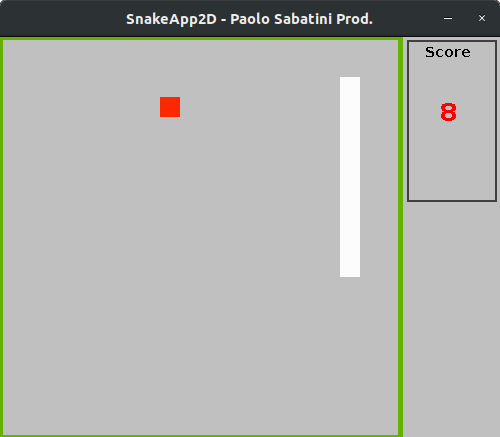
\includegraphics[width=0.42\textwidth]{imgs/SnakeScreen.png}
\caption{Screen of the game.}
\label{fig:game_screen}

\end{figure}

\newpage

\begin{thebibliography}{9}

\bibitem{MyGITHUB}
Paolo Sabatini,~\emph{BrainSnake: Reinforcement-trained AI vs Snake 2D},\\\href{https://github.com/paolosabatini/BrainSnake}{https://github.com/paolosabatini/BrainSnake}.

\bibitem{MyDOXYGEN}
Paolo Sabatini,~\emph{BrainSnake: Documentation of the BrainSnake project},\\ \href{https://paolosabatini.github.io/BrainSnake/}{https://paolosabatini.github.io/BrainSnake/}

\bibitem{GITHUB}
GitHub Inc.,~\href{https://github.com}{https://github.com}.

\bibitem{DOXYGEN}
Dimitri van Heesch,~\emph{Doxygen: Generate documentation from source code},\\\href{http://www.doxygen.org}{http://www.doxygen.org}

\bibitem{TRAVIS}
Travis~CI GmbH,~\emph{Travis CI: the simplest way to test and deploy your projects.},\\\href{https://travis-ci.com/}{https://travis-ci.com/}

\bibitem{SNAKE1}
Code Bullet,~\emph{I created the perfect Snake AI}, \\ \href{https://www.youtube.com/watch?v=tjQIO1rqTBE&t=1141s}{https://www.youtube.com/watch?v=tjQIO1rqTBE\&t=1141s}

\bibitem{SNAKE2}
Grer Viau,~\emph{Neural Network Learns to Play Snake},\\ \href{https://www.youtube.com/watch?v=zIkBYwdkuTk}{https://www.youtube.com/watch?v=zIkBYwdkuTk}

\bibitem{SNAKE3}
Elvis Sun,~\emph{Almost perfect Snake AI},\\ \href{https://www.youtube.com/watch?v=IJ-Cxsao040}{https://www.youtube.com/watch?v=IJ-Cxsao040}

\bibitem{SNAKE4}
AlphaPhoenix,~\emph{The unkillable Snake AI},\\ \href{https://www.youtube.com/watch?v=YqL7bl3I5IE}{https://www.youtube.com/watch?v=YqL7bl3I5IE}

\bibitem{SNAKE5}
Chispresso,~\emph{AI learns to play Snake},\\ \href{https://www.youtube.com/watch?v=vhiO4WsHA6c}{https://www.youtube.com/watch?v=vhiO4WsHA6c}

\bibitem{SNAKE6}
DeKay Arts,~\emph{How to automate Snake using Reinforcement Learning},\\ \href{https://www.youtube.com/watch?v=RMTfNPKnxhk}{https://www.youtube.com/watch?v=RMTfNPKnxhk}

\bibitem{JAVA}
Jan Bodnar,~\emph{Zetcode tutorial for Java 2D gaming},~\\ \href{http://zetcode.com/tutorials/javagamestutorial/}{http://zetcode.com/tutorials/javagamestutorial/} (2007 -- 2010).

\end{thebibliography}


\newpage
\begin{appendices}

\end{appendices}

\end{document}
